\chapter{Diseño e Implementación}
\label{sec:DisenoImplementacion}
Para implementar un sistema completo de \textit{Request To Pay}, se ha desarrollado un servidor HTTP que expone una API RESTful y un cliente web en tiempo real. El objetivo de este apartado es detallar cómo se ha llevado a cabo esta implementación, así como las fases de desarrollo involucradas.

\section{Fundamentos Teóricos}
Antes de profundizar en la implementación, es fundamental aclarar los dos pilares teóricos en los que se basa el sistema:

\begin{itemize}
    \item \textbf{Servidor HTTP}: Una aplicación que permanece a la escucha en un puerto de red, esperando conexiones TCP de clientes capaces de comunicarse mediante el protocolo HTTP. Una vez establecida la conexión, el servidor recibe un mensaje estructurado con los siguientes componentes:
    \begin{itemize}
        \item \textit{Línea de petición}: Indica el método (GET, POST, etc.), la ruta del recurso solicitado y la versión del protocolo.
        \item \textit{Cabeceras}: Aportan metadatos, como el tipo de contenido, credenciales o longitud del mensaje.
        \item \textit{Cuerpo} (opcional): Contiene datos adicionales, si el método lo requiere.
    \end{itemize}
    El servidor interpreta la ruta, determina qué componente interno debe procesarla, ejecuta la lógica correspondiente y genera una respuesta formada por:
    \begin{itemize}
        \item \textit{Línea de estado}: Incluye un código de resultado (por ejemplo, 200 OK, 404 Not Found, 500 Internal Server Error).
        \item \textit{Cabeceras}: Describen la respuesta.
        \item \textit{Cuerpo} (opcional): Contiene datos, como HTML o JSON.
    \end{itemize}
    Tras enviar la respuesta, la conexión puede cerrarse o mantenerse activa para futuras peticiones, dependiendo de la versión del protocolo y las cabeceras de control. En esencia, el servidor HTTP funciona como el centro de operaciones que recibe todas las solicitudes y coordina el acceso a la lógica y los datos de la aplicación.

    \item \textbf{API RESTful}: Se basa en los principios de la arquitectura REST (\textit{Representational State Transfer}\footnote{Transferencia de Estado Representacional}) aplicados al protocolo HTTP para exponer recursos de forma uniforme y predecible. Sus características principales son:
    \begin{itemize}
        \item Cada entidad del dominio (por ejemplo, un usuario o una petición RTP) se representa mediante una URL estable.
        \item Los verbos HTTP (POST, GET, PUT, DELETE) describen operaciones como creación, consulta, modificación o eliminación de recursos.
        \item El servidor es \textit{sin estado}, por lo que cada solicitud contiene toda la información necesaria, facilitando la escalabilidad horizontal.\footnote{Es decir, permite añadir o retirar servidores sin necesidad de compartir sesiones en memoria.}
        \item La uniformidad de los códigos de estado y los formatos de representación asegura que clientes heterogéneos consuman la API de manera predecible.
        \item Herramientas como cachés, control de versiones en URLs o cabeceras, y negociación de contenido permiten evolucionar la interfaz sin afectar a los consumidores existentes.
    \end{itemize}
\end{itemize}

En conjunto, el servidor HTTP actúa como el camino por donde viajan las solicitudes, mientras que la API RESTful establece las reglas claras y fáciles de mantener para que ese camino conecte eficientemente la lógica del servidor con los diversos clientes que dependen de ella.
%%%%%%%%%%%%%%%%%%%%%%%%%%%%%%%%%%%%%%%%%%%%%%%%%%%%%%%%%%%%%%%%%%%%%%%%%%%%%%%%%%%%%%%%%%%%%%%%%%%%%%%%%%%%%%%%%%
\section{Tecnologías utilizadas}
\label{subsec:Herramientas de desarrollo}
El desarrollo del proyecto se ha llevado a cabo en un entorno virtual Python que aísla las dependencias y permite reproducir la instalación mediante el comando \texttt{pip install -r requirements.txt}. Este enfoque asegura consistencia y portabilidad, facilitando tanto la colaboración entre desarrolladores como el despliegue en entornos diversos.

\textbf{Backend.} El núcleo del backend se fundamenta en Python 3 y Flask, un micro-framework que proporciona un servidor WSGI, un sistema de enrutado eficiente y una integración fluida con el estándar HTTP. Sobre esta base, se incorpora Flask-socketIO, un middleware que habilita la negociación de WebSockets, permitiendo servir tráfico HTTP y comunicación bidireccional en el mismo puerto de manera transparente. Para la gestión de datos, se emplea SQLAlchemy a través de Flask-SQLAlchemy, lo que facilita la representación de modelos de dominio como objetos Python, mientras que SQLite actúa como una base de datos ligera y autónoma durante el desarrollo, eliminando la necesidad de un servidor externo para transacciones básicas. Este núcleo se complementa con utilidades de la librería estándar de Python, incluyendo:
\begin{itemize}
    \item \texttt{hashlib}, para firmar transacciones de estado mediante el algoritmo SHA-256;
    \item \texttt{datetime}, para registrar marcas temporales en los logs.
\end{itemize}

\textbf{Frontend.} En el lado del cliente, se ha implementado un frontend estático basado en HTML5, CSS3 y JavaScript ES6, priorizando la ligereza al evitar frameworks complejos. La maquetación adaptativa se logra mediante Bootstrap 5, cargado vía CDN, y la iconografía se enriquece con Font Awesome, también distribuido por CDN. La comunicación en tiempo real se establece con el cliente Socket.IO 4.x, que conecta vía WebSocket al mismo host y puerto que Flask, mientras que las peticiones REST se realizan de forma nativa con la Fetch API, sin depender de librerías adicionales.

\textbf{Herramientas de desarrollo.} El entorno de trabajo se ha centrado en Visual Studio Code como editor principal, aprovechando sus extensiones para optimizar la gestión del proyecto y el desarrollo del código. El control de versiones se ha gestionado con Git, utilizando ramas específicas para cada funcionalidad nueva, lo que asegura un desarrollo ordenado y trazable. Para las pruebas manuales de la API, se ha empleado Postman, donde se diseñó una colección de peticiones parametrizadas que serán detalladas en secciones posteriores del documento.

El uso de un entorno virtual junto con dependencias consolidadas establece una base robusta para el despliegue de la aplicación en entornos más exigentes, como contenedores, nubes públicas o servidores locales, preservando la integridad de su arquitectura fundamental.
%%%%%%%%%%%%%%%%%%%%%%%%%%%%%%%%%%%%%%%%%%%%%%%%%%%%%%%%%%%%%%%%%%%%%%%%%%%%%%%%%%%%%%%%%%%%%%%%%%%%%%%%%%%%%%%%%%%%%%%%%%%%%%%
\section{Estructura y funcionamiento}
\label{subsec:Estructura}
El código del proyecto se estructura en dos componentes principales, \textbf{backend} y \textbf{frontend}, interconectados mediante los protocolos HTTP y WebSockets. Esta división, diseñada de manera intencionada, responde a la necesidad de lograr un desarrollo ordenado, eficiente y preparado para futuros crecimientos, considerando que trabajé en el proyecto de forma individual. Al separar el \textit{backend}, encargado de la lógica de negocio, el manejo de datos y la comunicación con el cliente, del \textit{frontend}, centrado en la interfaz de usuario y la experiencia interactiva, se obtiene una arquitectura clara y modular. Esta organización aporta múltiples ventajas: mejora la mantenibilidad al permitir identificar y corregir errores de manera localizada, simplifica la incorporación de nuevas funcionalidades sin alterar otras partes del sistema y refleja fielmente la arquitectura empleada en entornos de producción reales, lo que facilita una transición fluida hacia despliegues en contenedores, nubes públicas o servidores locales. Además, esta separación promueve la reutilización de código, ya que el \textit{backend} puede servir a múltiples clientes (como aplicaciones móviles o de escritorio) y el \textit{frontend} puede adaptarse a diferentes dispositivos sin modificar la lógica subyacente. A continuación, se describen los archivos que componen cada una de estas partes, su rol específico en el proyecto y el fragmento de código más relevante.

\begin{figure}[H]
  \centering
  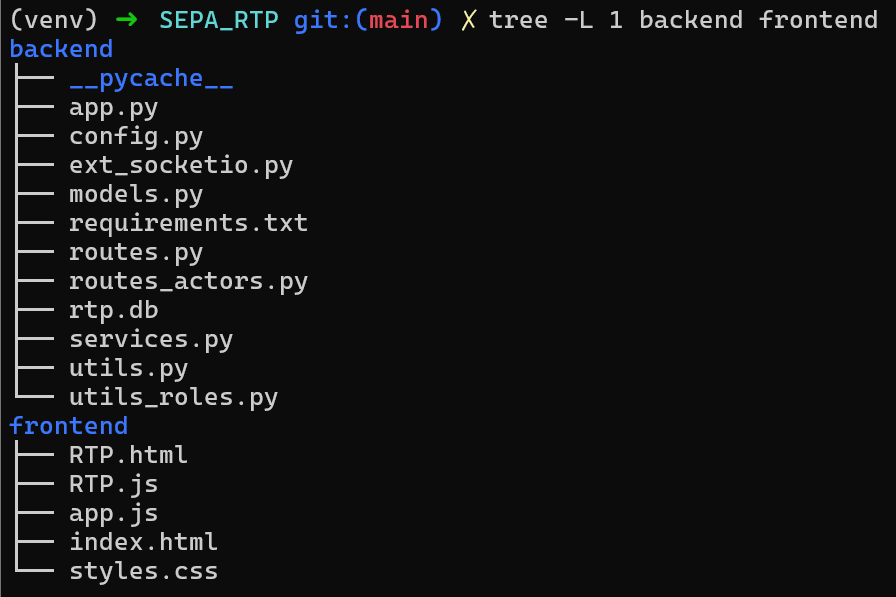
\includegraphics[width=0.8\textwidth]{Imagenes/treeB.png}
  \caption{Tree}
  \label{fig:Tree}
\end{figure}

\subsection{Backend}
\label{subsubsec:Backend}

\begin{itemize}
    \item \textbf{app.py} es el punto de arranque, para lanzar la aplicación debo ejecutar dentro de mi venv "python app.py". En este fichero se crea la instancia de Flask, aplica la configuración, inicializa la base de datos y arranca Socket.IO. Al mismo tiempo registra el blueprint con todos los endpoints y expone una ruta raíz que sirve directamente index.html, de manera que el mismo proceso pueda funcionar como servidor de APi y de archivos estáticos. 
        \begin{figure}[H]
            \centering
            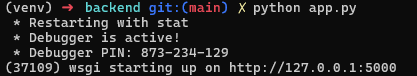
\includegraphics[width=0.8\textwidth]{Imagenes/Arranque1.png}
            \caption{Arranque}
            \label{fig:Arranque}
        \end{figure}
        Tras ejecutarlo basta con poner "http://127.0.0.1:5000"     en el buscador para conectarnos al servidor.


        \begin{lstlisting}[language=Python, style=custom, caption={Configuración y arranque del servidor Flask-SocketIO}]
            STATIC_FOLDER = os.path.join(os.path.dirname(__file__), '../frontend')
            app = Flask(__name__, static_folder=STATIC_FOLDER)
            app.config.from_object(Config)
            db.init_app(app)
            # Servir index.html en la raíz
            @app.route('/')
            def home():
                return app.send_static_file('index.html')

            # Servir archivos estáticos desde el directorio frontend
            @app.route('/<path:filename>')
            def serve_static(filename):
                return send_from_directory(app.static_folder, filename)

            # Registrar el blueprint con todos los endpoints de RTP
            app.register_blueprint(rtp_blueprint)

            @socketio.on('join')
            def handle_join(data):
                actor_id = data['actor_id']
                actor = Actor.query.get(actor_id)
                if actor:
                    room = f"{actor.role}_{actor_id}"
                    join_room(room)
                    print(f"Actor {actor_id} se unió a la sala {room}")

            if __name__ == '__main__':
                webbrowser.open("http://127.0.0.1:5000/")
                socketio.run(app, debug=True)
        \end{lstlisting}

    \item \textbf{config.py} contiene la configuración: URI de SQLite y parámetro para desactivar el tracker de SQLAlchemy. Facilita cambiar de motor BD en modificaciones futuras solamente cambiando esta clase.
            \begin{lstlisting}[language=Python, style=custom, caption={Configuración SQLAlchemy y SQLite}]
                basedir = os.path.abspath(os.path.dirname(__file__))

                class Config:
                    SQLALCHEMY_DATABASE_URI = 'sqlite:///' + os.path.join(basedir, 'rtp.db')
                    SQLALCHEMY_TRACK_MODIFICATIONS = False

            \end{lstlisting}

    \item \textbf{models.py} define el modelo de datos que se va utilizar y contiene un ORM\footnote{Object-Relational Mapping} para interactuar con una base de datos relacional. Aquí definimos tres clases principales que representan tablas en la base de datos: Actor, RTP y log.
            Esto se hace así para mayor facilidad a la hora de realizar operaciones como crear, leer, actualizar y eliminar registros.
            Cada una de estas clases corresponde con una tabla en la base de datos y cada atributo de cada clase con una columna de su tabla correspondiente. Además se incluye un método todict para serializar los datos a formato JSON para enviarlos a través de una API.
            A continuacion se muestra únicamente una de las 3 clases ya que ambas tienen la misma estructura.

            \begin{lstlisting}[language=Python, style=custom, caption={Modelo ORM + clase Actor}]
                    from flask_sqlalchemy import SQLAlchemy

                    db = SQLAlchemy()

                    class Actor(db.Model):
                        __tablename__ = 'actor'
                        id = db.Column(db.Integer, primary_key=True)
                        username = db.Column(db.String(50), unique=True)
                        password = db.Column(db.String(50))
                        name = db.Column(db.String(50), nullable=False)
                        role = db.Column(db.String(20), nullable=False)

                        photo_url = db.Column(db.String(200), nullable=True)  # URL o base64
                        iban = db.Column(db.String(34), nullable=True)
                        balance = db.Column(db.Float, default=0.0)

                        # Campo nuevo: psp_id, que referencia a otro Actor que es PSP
                        psp_id = db.Column(db.Integer, db.ForeignKey('actor.id'), nullable=True)
                        # Relación para que se pueda acceder con actor.psp
                        psp = db.relationship('Actor', remote_side=[id])

                        def to_dict(self):
                            return {
                                "id": self.id,
                                "username": self.username,
                                "name": self.name,
                                "role": self.role,
                                "photo_url": self.photo_url,
                                "iban": self.iban,
                                "balance": self.balance,
                                "psp_id": self.psp_id  # Podríamos incluir más info del psp, etc.
                            }

                \end{lstlisting}

    \item \textbf{utils.py} agrega métodos auxiliares que son llamados desde otros ficheros. Son métodos de utilidad y se han puesto en este fichero con el objetivo de no sobrecargar los ficheros principales. Algunas de las funcionalidades que incluye son "cambiar\_esatdo_rtp", "rechazar\_rtp" o "validar\_iban".

            \begin{lstlisting}[language=Python, style=custom, caption={Funciones utilitarias}]
                def cambiar_estado_rtp(db, rtp_obj, new_status):
                old_status = rtp_obj.status
                rtp_obj.status = new_status
                db.session.commit()

                # Generar un hash
                hash_input = f"{rtp_obj.id}{rtp_obj.iban}{rtp_obj.amount}{old_status}{new_status}".encode('utf-8')
                hash_value = hashlib.sha256(hash_input).hexdigest()

                nuevo_log = Log(
                    rtp_id=rtp_obj.id,
                    old_status=old_status,
                    new_status=new_status,
                    hash_value=hash_value
                )
                db.session.add(nuevo_log)
                db.session.commit()

                return {
                    "message": f"RTP {rtp_obj.id} actualizado de {old_status} a {new_status}"
                }

            def rechazar_rtp(db, rtp_obj, motivo):
                return cambiar_estado_rtp(db, rtp_obj, "rechazado")

            def validar_iban(iban, rtp_obj):
                iban = rtp_obj.iban
                if not iban or not isinstance(iban, str) or len(iban) < 15:
                    return cambiar_estado_rtp(db, rtp_obj, "rechazado")
                if not (iban[:2].isalpha() and iban[2:].replace(' ', '').isalnum()):
                    return cambiar_estado_rtp(db, rtp_obj, "rechazado")
                return {
                    "message": f"RTP {rtp_obj.id} validado con IBAN correcto"
                }

            \end{lstlisting}

    \item \textbf{utils roles.py} contiene el decorador rolerequired que inspecciona el actorid recibido en el cuerpo JSON y bloquea la ruta si el rol no coincide con el requerido.
            De esta manera se asegura de cada actor tenga acceso a sus propias funciones.

            \begin{lstlisting}[language=Python, style=custom, caption={Decorador para control de funciones}]
                def role_required(required_role):
                """
                Decorador que verifica que el actor que invoca el endpoint
                tenga el rol adecuado.
                Se espera que en el body JSON llegue "actor_id".
                """
                def decorator(f):
                    @wraps(f)
                    def wrapper(*args, **kwargs):
                        data = request.get_json() or {}
                        actor_id = data.get('actor_id')
                        if not actor_id:
                            return jsonify({"error": "Se requiere actor_id para esta acción"}), 400

                        actor = Actor.query.get(actor_id)
                        if not actor:
                            return jsonify({"error": "Actor no encontrado"}), 404

                        if actor.role != required_role:
                            return jsonify({"error": f"Rol '{actor.role}' no tiene acceso a esta acción"}), 403

                        # Si el rol coincide, continuamos
                        return f(*args, **kwargs)
                    return wrapper
                return decorator

            \end{lstlisting}
    
    \item \textbf{services.py} contiene la capa de negocio. Cada función del fichero orquesta la consulta/actualizacion de modelos, invoca las utilidades de estado y emite eventos Socket.IO a la room adecuada.
            A través de todas estas funciones se lleva a cabo el flujo RTP, que posteriormente explicaré.
    
    \item \textbf{routes.py} contiene el Blueprint que expone la máquina de estados RTP (cinco rutas POST) y utilidades de autenticación, perfil y logs. Cada endpoint invoca a su homónimo en servcies.py y devuelve el JSON estandarizado.
            Algunas de estos endpoints que no afectan directamente sobre el flujo RTP son el proceso de login (ya que se trata de simular la página de un banco) o el apartado de perfil donde puedes modificar algunos elementos.

            A cada uno de estos endpoints le corresponde su fichero o apartado .html que veremos en posteriores apartados del documento.
            
            \begin{lstlisting}[language=Python, style=custom, caption={Declaración blueprint rtp}]
                rtp_blueprint = Blueprint('rtp', __name__)
            \end{lstlisting}

            \begin{lstlisting}[language=Python, style=custom, caption={Endpoint login}]
                @rtp_blueprint.route('/login', methods=['POST'])
                def login():
                    data = request.get_json()
                    username = data.get('username')
                    password = data.get('password')
                    if not username or not password:
                        return jsonify({"error": "Faltan credenciales"}), 400
                    
                    actor = Actor.query.filter_by(username=username).first()
                    if not actor:
                        return jsonify({"error": "Usuario no existe"}), 404
                    
                    if actor.password != password:
                        return jsonify({"error": "Contraseña incorrecta"}), 401
                    
                    # Login exitoso
                    return jsonify({
                        "message": "Login correcto",
                        "actor_id": actor.id,
                        "role": actor.role,
                        "name": actor.name
                    })
            \end{lstlisting}

            \begin{lstlisting}[language=Python, style=custom, caption={Endpoint profile}]
                    @rtp_blueprint.route('/profile', methods=['POST'])
                    @role_required('payer')
                    def update_profile():
                        data = request.get_json() or {}
                        actor_id = data.get('actor_id')
                        actor = Actor.query.get(actor_id)
                        if not actor:
                            return jsonify({"error": "Actor no encontrado"}), 404

                        # Campos opcionales
                        new_photo = data.get('photo_url')
                        new_iban = data.get('iban')
                        new_balance = data.get('balance')

                        if new_photo is not None:
                            actor.photo_url = new_photo
                        if new_iban is not None:
                            actor.iban = new_iban
                        if new_balance is not None:
                            actor.balance = float(new_balance)

                        db.session.commit()
                        return jsonify({"message": "Perfil actualizado", "actor": actor.to_dict()})

            \end{lstlisting}

    \item \textbf{routes actors.py} contiene un pequeño blueprint aparte para el alta de actores, esto se ha hecho así para demostrar cómo escalar la API sin engordar el fichero principal.
            \begin{lstlisting}[language=Python, style=custom, caption={Declaración blueprint actores}]
                actors_blueprint = Blueprint('actors', __name__)

                @actors_blueprint.route('/actors', methods=['POST'])
                def create_actor():
                    data = request.get_json()
                    name = data.get('name')
                    role = data.get('role')  # 'beneficiary', 'psp_beneficiary', 'psp_payer', 'payer'

                    if not name or not role:
                        return jsonify({"error": "Faltan campos requeridos: name, role"}), 400

                    # Validar que el role sea uno de los cuatro permitidos:
                    valid_roles = ['beneficiary', 'psp_beneficiary', 'psp_payer', 'payer']
                    if role not in valid_roles:
                        return jsonify({"error": f"Rol '{role}' no válido"}), 400

                    actor = Actor(name=name, role=role)
                    db.session.add(actor)
                    db.session.commit()

                    return jsonify({"message": "Actor creado", "id": actor.id, "role": actor.role}), 201

            \end{lstlisting}

    \item \textbf{ext socketio.py} simplemente es un fichero de conveniencia que crea la instancia soccketIO.
            Separar la instancia de Socket.IO en un fichero independiente permite mantener una arquitectura limpia y flexible: evita importaciones circulares entre módulo, se integra sin fricción en el patrón application factory de Flask al poder llamarse luego socketio.initapp desde app.py. Así centralizamos en un único punto la configuración o el cambio de motor de concurrencia facilitando la escalabilidad.
            \begin{lstlisting}[language=Python, style=custom, caption={Instancia global de socketIO}]
                from flask_socketio import SocketIO, join_room, emit

                socketio = SocketIO()
            \end{lstlisting}


    \item \textbf{rtp.db} es una base de datos sencilla que se crea sola la primera vez que inicias la aplicación. Cuando arrancas el programa, las herramientas explicadas anteriormente crean este archivo automáticamente. Este archivo guarda toda la información del proyecto, como las tablas y datos, sin necesidad de instalar nada más ni usar un servidor aparte. Esto hace que sea muy fácil empezar a trabajar en el proyecto, ya sea para desarrollarlo, hacer pruebas o mostrar cómo funciona, porque solo necesitas instalar lo básico.

        Cuando el proyecto crezca y se necesite manejar más usuarios al mismo tiempo, hacer copias de seguridad mientras está funcionando o tener varias copias de la base de datos, se puede cambiar a una base de datos más potente, como PostgreSQL o MySQL. Esto se hace simplemente cambiando una dirección de conexión, sin modificar casi nada del programa.
\end{itemize}

\subsection{Frontend}
\label{subsubsec:Frontend}

\begin{itemize}
    \item \textbf{index.html} define el formulario de login inicial, el navbar colapsable y cinco bloques: homeDashboard, seccionCuentas, seccionTarjetas, seccionPerfiles y seccionRTP, de las cuales la única relevante es la seccionRTP, las demás son relleno para simular una página de un banco.
        
    El documento carga Bootstrap 5, Font Awesome, Google Fonts y la hoja styles.css.

    Al final del documento se incluye app.js y RTP.js de modo que la misma página sirve toda la experiencia de usuario sin recargas.
    \item \textbf{app.js} desempeña un papel central como el núcleo de la interfaz de usuario, orquestando toda la experiencia de la aplicación de página única (\textit{single-page application}, SPA) del proyecto. Desde su carga inicial, este fichero establece las bases para una interacción fluida y dinámica, integrando las siguientes funcionalidades clave:
        \begin{itemize}
            \item \textbf{Establecimiento de la conexión WebSocket.} Al cargarse, inicia una conexión WebSocket con el servidor mediante una instrucción adecuada, asegurando que los eventos emitidos por el backend lleguen al navegador en tiempo real. Tras un inicio de sesión exitoso, envía un evento \texttt{join} que suscribe al usuario a la sala correspondiente, permitiendo recibir actualizaciones instantáneas de cambios de estado.

            \item \textbf{Gestión del proceso de autenticación.} Intercepta el envío del formulario de inicio de sesión, realiza una solicitud \texttt{POST /login}, almacena en memoria el identificador (\texttt{currentActorId}) y el rol (\texttt{currentActorRole}) devueltos por la API, y desbloquea la navegación por la aplicación, ofreciendo una transición suave al usuario.

            \item \textbf{Navegación tipo SPA.} Incluye una función que muestra u oculta secciones según la opción seleccionada en la barra de menús, evitando recargas completas de la página y simulando la experiencia de una aplicación nativa. Esta funcionalidad garantiza una navegación ágil y eficiente.

            \item \textbf{Carga del panel principal.} Al acceder al panel "Inicio", invoca un cargador de datos que obtiene el perfil del usuario mediante una solicitud \texttt{fetch}, formatea el saldo con separadores de miles para mayor claridad, enmascara el IBAN por razones de seguridad y ajusta dinámicamente el tamaño de fuente para que el monto se ajuste perfectamente dentro del círculo de balance.

            \item \textbf{Edición del perfil.} Ofrece un módulo que precarga el formulario con los datos actuales del usuario, permite su edición y, al enviarlo, actualiza la información en el servidor a través de una solicitud \texttt{POST /profile}, mostrando mensajes de éxito o error sin necesidad de salir de la página.

            \item \textbf{Adaptación a dispositivos móviles.} Monitorea los eventos de expansión y colapso de la barra de navegación (\textit{navbar}) de Bootstrap, ajustando la visibilidad del menú inferior para evitar que los controles oculten el contenido en pantallas pequeñas, asegurando una experiencia coherente y usable.

            \item \textbf{Mantenimiento del estado y sincronización.} Coordina el estado del usuario, sincroniza los datos con el backend, responde a notificaciones en tiempo real y proporciona una navegación fluida, todo ello sin depender de frameworks SPA pesados. Incluye utilidades propias como funciones para formatear cantidades, IBANs y tamaños de texto, que refuerzan la usabilidad y la consistencia visual de la aplicación.
        \end{itemize}

    \item \textbf{RTP.js} se encarga de transformar la sección RTP de la aplicación de página única (\textit{single-page application}, SPA) en un panel interactivo que opera en tiempo real. Este módulo integra la interfaz visual con el backend, gestiona eventos dinámicos y ofrece flujos de trabajo adaptados a los roles de los usuarios, todo ello mientras mantiene un diseño ligero y sin dependencias de frameworks externos. A continuación, se detallan sus principales funcionalidades:
    
        \begin{itemize}
            \item \textbf{Carga inicial de la interfaz.} Una vez que el DOM está completamente cargado, el módulo descarga el fragmento \texttt{RTP.html} y lo inserta en el contenedor \texttt{seccionRTP}. Posteriormente, invoca un inicializador que registra los \textit{event listeners} necesarios para la interacción. Este enfoque mantiene el HTML de la interfaz separado del código JavaScript, lo que reduce el peso de la página principal y facilita el mantenimiento.

            \item \textbf{Gestión de notificaciones y roles.} \texttt{RTP.js} almacena en memoria un arreglo con todas las notificaciones recibidas durante la sesión del usuario. Utilizando la variable global \texttt{currentActorRole}, determina qué panel de acciones debe mostrarse (Beneficiario, PSP Beneficiario, PSP Pagador o Pagador) y oculta los demás. Esta lógica de visibilidad se aplica tanto al cargar la sección como al cambiar de pestaña, asegurando que la interfaz se adapte dinámicamente al rol del usuario, incluso si la sesión se reutiliza para diferentes perfiles.

            \item \textbf{Flujos de trabajo por rol.} El módulo encapsula los procesos de negocio mediante manejadores de eventos que varían según el rol del usuario:
            \begin{itemize}
                \item \textit{Beneficiario}: Intercepta el formulario "Crear RTP", construye un objeto JSON con el IBAN, el importe y el identificador del actor, y lo envía a \texttt{POST /rtp}. La respuesta del servidor se muestra en un contenedor de retroalimentación.
                \item \textit{PSP Beneficiario}: Proporciona formularios para validar al beneficiario (\texttt{POST /rtp/\linebreak <id>/validate-beneficiary}) y enrutar la solicitud (\texttt{POST /rtp/<id>/route}).
                \item \textit{PSP Pagador}: Ofrece un formulario para validar los fondos del pagador.
                \item \textit{Pagador}: Incluye un formulario para tomar la decisión final (aceptar o rechazar la solicitud).
            \end{itemize}
            Cada acción se realiza mediante la API Fetch sin recargar la página, y los resultados se notifican visualmente al usuario. Además, los identificadores RTP pueden accionarse desde botones en la tabla de notificaciones, permitiendo a PSPs y pagadores responder con un solo clic, sin necesidad de completar formularios manualmente.

            \item \textbf{Sincronización en tiempo real.} El módulo instala \textit{listeners} WebSocket para los eventos \texttt{rtp\_created}, \texttt{rtp\_routed}, \texttt{rtp\_validated\_payer} y \texttt{rtp\_decision}. Cuando el backend emite uno de estos eventos, el cliente verifica si el rol conectado es el destinatario. Si lo es, añade el objeto RTP al arreglo de notificaciones y actualiza la tabla de la interfaz. El renderizado genera filas con el importe, el estado y un botón contextual que activa la acción correspondiente según el rol y el estado actual, manteniendo la interfaz sincronizada sin necesidad de solicitudes adicionales al servidor.

            \item \textbf{Auditoría de transacciones.} Un botón ``Mostrar logs'' realiza una solicitud \texttt{GET /logs}, recupera el historial de transiciones firmado con SHA-256 y lo presenta en un listado colapsable. Esto permite al usuario revisar el ciclo de vida de cada solicitud de manera instantánea, ofreciendo una herramienta de auditoría clara y accesible.
        \end{itemize}

    \item \textbf{RTP.html} es una plantilla HTML autónoma que el cliente carga dinámicamente cuando el usuario accede a la sección Request-to-Pay; reúne, en un único fragmento, los formularios de acción de los cuatro roles (Beneficiary, PSP Beneficiary, PSP Payer y Payer) y una tabla de notificaciones donde se van listando los cambios de estado recibidos en tiempo real, de modo que toda la interfaz específica del flujo RTP se mantiene separada del documento principal y puede insertarse o actualizarse sin recargar la página.
    \item \textbf{styles.css} es consumido por todas las páginas del frontend (por ejemplo, index.html y los fragmentos dinámicos como RTP.html) y su única misión es dotar de coherencia visual a la aplicación: define la paleta de colores (degradados morados y dorados), las tipografías (Montserrat y Great Vibes), los espaciados y sombras de los componentes (cards, inputs, botones), y aplica transiciones suaves (hover, fade-in) para mejorar la percepción de interactividad sin añadir ninguna lógica de negocio. 
\end{itemize}

\section{Emulación del prototipo \textit{Request To Pay}}
\label{subsec:EmulacionRTP}
Para emular el flujo Request To Pay, se han configurado cuatro actores con roles y permisos claramente diferenciados: el beneficiario, el pagador y los PSP correspondientes a cada uno de ellos. Cada actor dispone de un conjunto específico de endpoints REST para ejecutar sus operaciones (crear, validar, enrutar y decidir sobre una petición RTP) y escucha eventos WebSocket que garantizan la notificación en tiempo real de cada cambio de estado. De esta manera, el sistema reproduce fielmente el ciclo completo de una solicitud de cobro, desde su emisión por parte del beneficiario hasta la decisión final del pagador, manteniendo la trazabilidad y la coherencia de los estados en el backend y el frontend.

Tal como se describió anteriormente, todos los participantes deben estar previamente registrados en el Registro OSM, que actúa como fuente única de verdad y coordina la relación entre clientes y sus proveedores de servicio de pago. Gracias a este repositorio central, el banco del pagador ya conoce a su cliente y, de forma análoga, el banco del beneficiario está al tanto de su cliente beneficiario. Cuando este último genera una solicitud RTP introduciendo el IBAN del pagador, el OSM suministra automáticamente la información del PSP correspondiente, de modo que la petición se dirige al servicio adecuado. Por tanto, en esta emulación se asume la inscripción previa de los actores en el OSM y no se modela el proceso de registro dentro del flujo RTP.

Cuando ejecuto el código y me conecto al servidor lo que se ve es la página del login. Esto emula el proceso de login de la página web o aplicación de un banco real, en la cual si no eres cliente, no puedes acceder.

\begin{figure}[H]
  \centering
  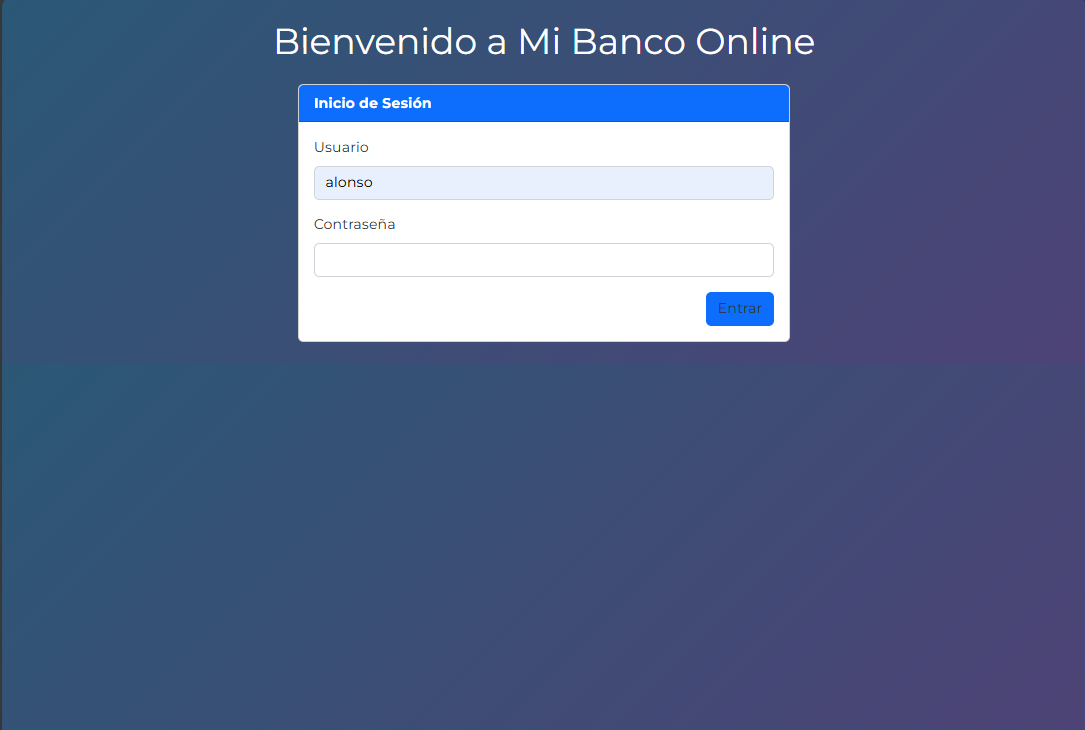
\includegraphics[width=0.8\textwidth]{Imagenes/LoginForm.png}
  \caption{LoginForm}
  \label{fig:Login}
\end{figure}

Tras iniciar sesión, la aplicación muestra la \textbf{página principal del banco} (Figura \ref{fig:DashBoard}) con los datos esenciales del cliente —nombre, IBAN, saldo y fotografía— y un menú superior que da acceso a funcionalidades habituales como \emph{Cuentas}, \emph{Tarjetas} o \emph{Perfil}. Esta interfaz reproduce la estética y el flujo de una banca en línea real: si no eres cliente, el proceso se detiene en la pantalla de inicio de sesión; si lo eres, se habilitan los paneles correspondientes a tus productos financieros.

\begin{figure}[H]
  \centering
  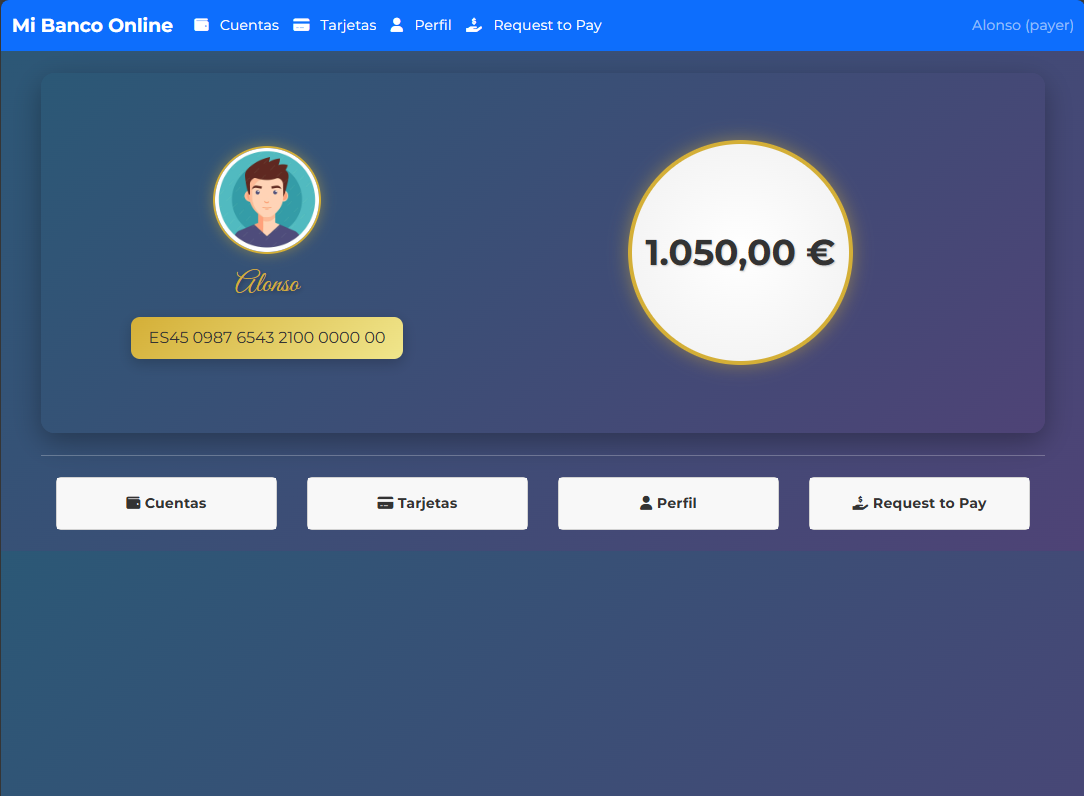
\includegraphics[width=0.8\textwidth]{Imagenes/DashBoard.png}
  \caption{DashBoard}
  \label{fig:DashBoard}
\end{figure}

Lo verdaderammente novedoso del prototipo, y por tanto, el \emph{producto} que se "vende" es la nueva opcion \emph{Request To Pay} que aparece en el menú. Dicha opción encapsula todo el software desarrollado ya explicado anteriormente.

La propuesta es que, una vez los bancos se adhieran al esquema RTP, todas las webs y aplicaciones bancarias incorporen esta sección tal y como se muestra aquí. El módulo es independiente, integrable vía API y compatible con las plataformas existentes, de manera que cualquier entidad que se registre en el sistema podría habilitarlo sin rediseñar su banca digital. En síntesis el producto de este TFG es un software que materializa el estándar RTP y lo hace accesible al usuario final desde la misma pantalla donde hoy consulta su saldo o sus tarjetas.

Como el objeto de interés es el apartado RTP el resto de apartados son secciones vacías ya que no aportan nada:

\begin{figure}[H]
  \centering
  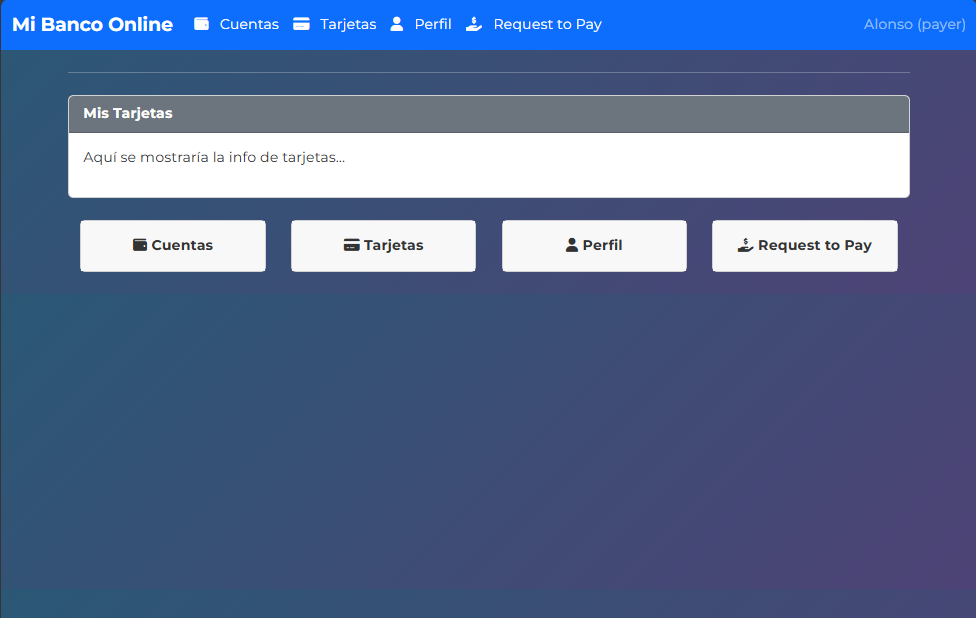
\includegraphics[width=0.8\textwidth]{Imagenes/Tarjetas.png}
  \caption{Tarjetas}
  \label{fig:Tarjetas}
\end{figure}

\begin{figure}[H]
  \centering
  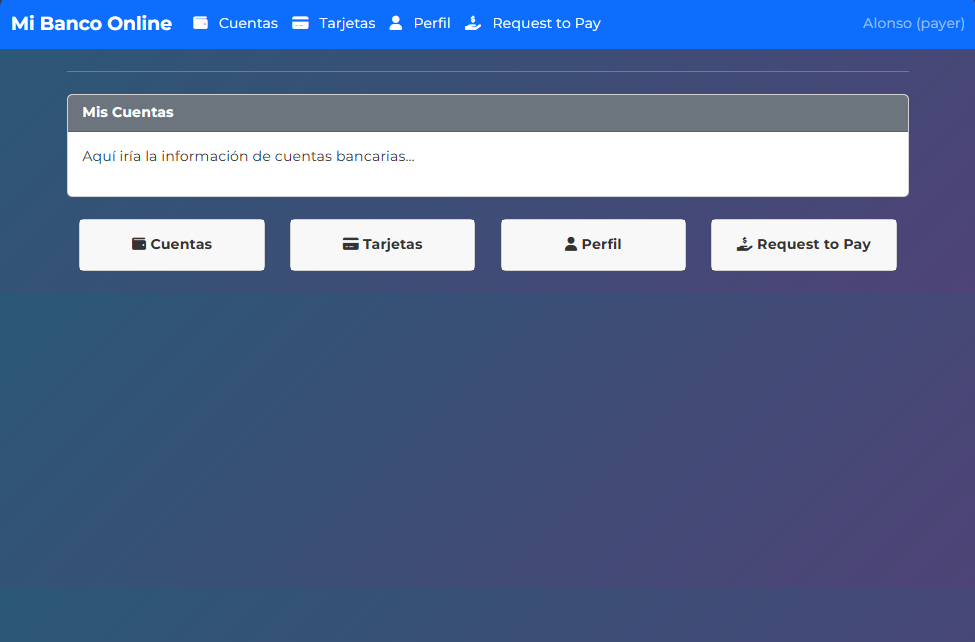
\includegraphics[width=0.8\textwidth]{Imagenes/Cuentas.png}
  \caption{Cuentas}
  \label{fig:Cuentas}
\end{figure}

En la opción Perfil se pueden consultar o modificar algunos datos.

\begin{figure}[H]
  \centering
  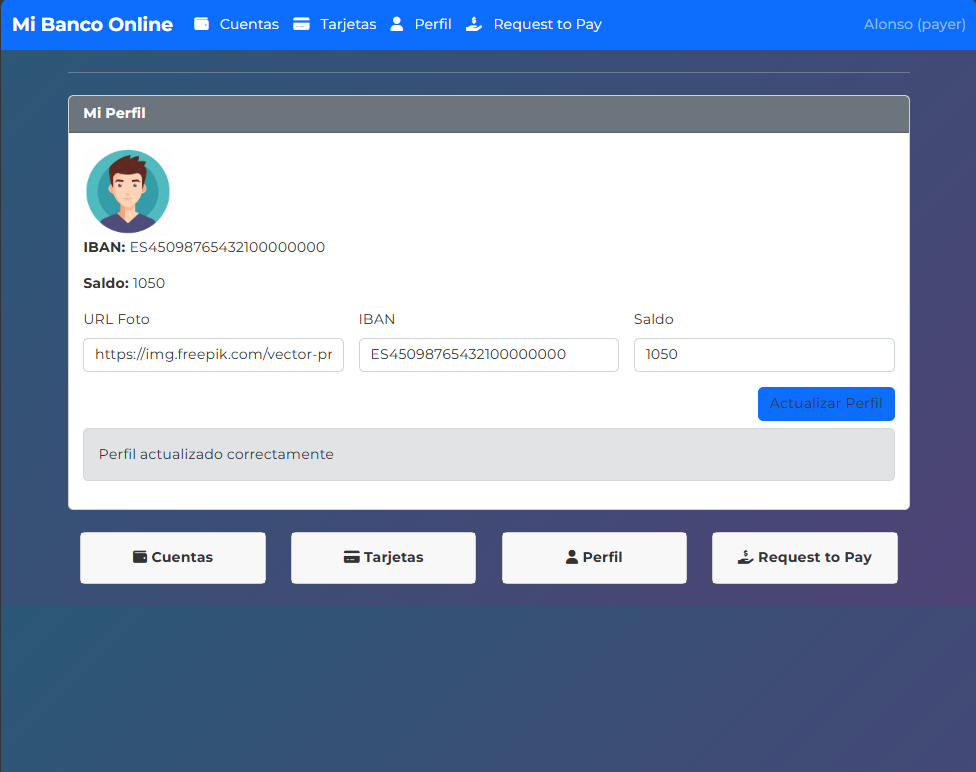
\includegraphics[width=0.8\textwidth]{Imagenes/Perfil.png}
  \caption{Perfil}
  \label{fig:Perfil}
\end{figure}

Esto aplica a todos los usuarios registrados en la página del banco, tanto empresas como clientes.

A continuación voy a explicar cómo se modela el flujo de un proceso de pago mediante RTP. En primer lugar he iniciado sesión en la página del banco de los cuatro actores para ser conscientes de qué es lo que vería cada uno de ellos durante el proceso.

Me centraré en explicar principalmente el backend, ya que el frontend es una página web y no creo que haya que detallar demasiado.

\begin{itemize}
    \item \textbf{Creación del RTP}\\[6pt]
        El flujo comienza cuando el beneficiario, ya autenticado, envía una
        petición \texttt{POST} a la ruta \texttt{/rtp}.  
        A partir de aquí intervienen dos piezas de código: la capa de
        exposición HTTP y la capa de negocio que materializa la petición.
        \vspace{0.6em}

        %---------------------------------------------------------------
        % 1. Endpoint HTTP (routes.py)
        %---------------------------------------------------------------
       \begin{lstlisting}[language=Python, style=custom, caption={Endpoint creación de solicitud RTP}]
            @rtp_blueprint.route('/rtp', methods=['POST'])
            @role_required('beneficiary')
            def crear_rtp():
                data = request.get_json()
                # ID del beneficiario que está logueado
                beneficiary_id = data.get('actor_id')
                # IBAN del pagador
                payer_iban = data.get('payer_iban')
                # Importe solicitado
                amount = data.get('amount')

                if not payer_iban:
                    return jsonify({"error": "Falta iban"}), 400

                if not amount:
                    return jsonify({"error": "Falta amount"}), 400

                # Delegación a la capa de negocio
                result = crear_rtp_service(data)
                status = 201 if "error" not in result else 400
                return jsonify(result), status
        \end{lstlisting}

        \begin{enumerate}
           \item Se impone un control de acceso que restringe la ruta a
                 beneficiarios.  
           \item Se extraen y validan los tres datos imprescindibles:
                 identificador del beneficiario, IBAN del pagador e importe.  
           \item Si alguno falta, se aborta el flujo devolviendo un error de
                 validación.  
           \item Con los datos verificados, la lógica de negocio toma el
                 relevo y, al finalizar, la ruta convierte su resultado en una
                 respuesta HTTP adecuada (éxito o error).
        \end{enumerate}
        \vspace{0.8em}

        %---------------------------------------------------------------
        % 2. Lógica de negocio (services.py)
        %---------------------------------------------------------------
       \begin{lstlisting}[language=Python, style=custom, caption={Servicio de negocio creacion RTP}]

            def crear_rtp_service(data):
                beneficiary_id = data.get('actor_id')
                payer_iban      = data.get('payer_iban')
                amount          = data.get('amount')

                # 1) Validar beneficiario y su PSP
                beneficiary = Actor.query.get(beneficiary_id)
                if not beneficiary or beneficiary.role != 'beneficiary':
                    return {"error": "El actor no es beneficiario o no existe"}

                if not beneficiary.psp_id:
                    return {"error": "El beneficiario no tiene PSP asociado"}
                psp_benef_id = beneficiary.psp_id

                # 2) Localizar pagador y su PSP
                payer = Actor.query.filter_by(iban=payer_iban, role='payer').first()
                if not payer:
                    return {"error": "No se encontró un pagador con ese IBAN"}

                if not payer.psp_id:
                    return {"error": "El pagador no tiene PSP asociado"}
                psp_payer_id = payer.psp_id

                # 3) Crear y guardar el RTP
                nuevo_rtp = RTP(
                    iban=payer_iban,
                    amount=amount,
                    beneficiary_id=beneficiary.id,
                    psp_beneficiary_id=psp_benef_id,
                    psp_payer_id=psp_payer_id,
                    payer_id=payer.id
                )
                db.session.add(nuevo_rtp)
                db.session.commit()

                # 4) Notificación en tiempo real al PSP del beneficiario
                socketio.emit(
                    'rtp_created',
                    nuevo_rtp.to_dict(),
                    room=f'psp_beneficiary_{psp_benef_id}'
                )

                return {
                    "message": "RTP creado correctamente",
                    "id": nuevo_rtp.id
                }
        \end{lstlisting}

        \begin{enumerate}
          \item Se verifica que el beneficiario existe, posee el rol correcto
                y tiene un PSP asignado.  
          \item Se identifica al pagador mediante su IBAN y se confirma que
                también cuenta con un PSP registrado.  
          \item Una vez validados ambos actores y sus PSP, se crea un registro
                RTP que deja constancia de todos los datos relevantes y se
                persiste en la base de datos.  
          \item Al confirmarse la grabación, se emite un evento en tiempo real
                dirigido al canal del PSP del beneficiario, de modo que este
                recibe instantáneamente la solicitud y puede empezar a
                procesarla.
        \end{enumerate}
        \bigskip

        Gracias a la coordinación entre estos dos bloques de código el primer
        paso del flujo Request~To~Pay queda cubierto: la petición se registra
        de forma duradera y el PSP del beneficiario obtiene la información
        necesaria para continuar con las etapas siguientes.

    \item \textbf{Validación y enrutamiento del RTP por parte del PSP beneficiario}\\[6pt]
        Una vez que el beneficiario ha creado el RTP y el PSP del beneficiario ha
        recibido la notificación, este PSP asume el control para verificar la
        solicitud y, si todo es correcto, remitirla al PSP del pagador.
        \vspace{0.6em}

        %---------------------------------------------------------------
        % 1. Endpoints HTTP (routes.py)
        %---------------------------------------------------------------
       \begin{lstlisting}[language=Python, style=custom, caption={Endpoints para validación y enrutado}]
            @rtp_blueprint.route('/rtp/<int:rtp_id>/validate-beneficiary', methods=['POST'])
            @role_required('psp_beneficiary')
            def validar_beneficiario(rtp_id):
                result = validar_beneficiario_service(rtp_id)
                status = 200 if "error" not in result else 400
                return jsonify(result), status

            @rtp_blueprint.route('/rtp/<int:rtp_id>/route', methods=['POST'])
            @role_required('psp_beneficiary')
            def enrutar_rtp(rtp_id):
                result = enrutar_rtp_service(rtp_id)
                status = 200 if "error" not in result else 400
                return jsonify(result), status
        \end{lstlisting}

        \begin{enumerate}
          \item \emph{Control de acceso}.  
                Ambas rutas están protegidas para garantizar que sólo un actor
                con rol de PSP del beneficiario pueda ejecutar estas acciones.
          \item \emph{Validación inicial}.  
                La primera ruta confirma que el RTP cumple los requisitos
                mínimos (coherencia de datos, existencia, formato, seguridad).
                Si la verificación falla, se devuelve un error; en caso
                contrario, el proceso avanza.
          \item \emph{Enrutamiento}.  
                La segunda ruta, accesible tras la validación, pone el RTP en
                camino hacia el PSP del pagador, devolviendo una respuesta de
                éxito cuando la operación se completa o un error si surge
                alguna incidencia.
        \end{enumerate}
        \vspace{0.8em}

        %---------------------------------------------------------------
        % 2. Lógica de negocio (services.py)
        %---------------------------------------------------------------
       \begin{lstlisting}[language=Python, style=custom, caption={Servicio de negocio validación y enrutado}]
            def validar_beneficiario_service(rtp_id):
                rtp_obj = RTP.query.get(rtp_id)
                if not rtp_obj:
                    return {"error": "RTP no encontrado"}
                result = cambiar_estado_rtp(db, rtp_obj, "validado-beneficiario")

                socketio.emit(
                    'rtp_validated_beneficiary',
                    rtp_obj.to_dict(),
                    room=f'psp_beneficiary_{rtp_obj.psp_beneficiary_id}'
                )
                return result

            def enrutar_rtp_service(rtp_id):
                rtp_obj = RTP.query.get(rtp_id)
                if not rtp_obj:
                    return {"error": "RTP no encontrado"}
                result = cambiar_estado_rtp(db, rtp_obj, "enrutado")

                socketio.emit(
                    'rtp_routed',
                    rtp_obj.to_dict(),
                    room=f'psp_payer_{rtp_obj.psp_payer_id}'
                )
                return result
        \end{lstlisting}
        \begin{enumerate}
          \item \emph{Recuperación y comprobación}.  
                Para cada operación se localiza el registro RTP mediante su
                identificador y se verifica su existencia; de no hallarse, se
                informa del error.
          \item \emph{Actualización de estado}.  
                \begin{itemize}
                  \item En la validación se marca el RTP como
                        \texttt{validado-beneficiario}.  
                  \item En el enrutamiento se actualiza a
                        \texttt{enrutado}, indicando que ya ha sido
                        despachado hacia el PSP del pagador.
                \end{itemize}
          \item \emph{Persistencia}.  
                Cada cambio de estado se registra de forma duradera en la base
                de datos, lo que asegura la trazabilidad del flujo.
          \item \emph{Notificación en tiempo real}.  
                Tras la validación se emite un evento dirigido a la sala del
                propio PSP beneficiario para confirmar la operación; después,
                al enrutarse, se envía otro evento a la sala del PSP del
                pagador, de modo que este último reciba de inmediato la
                solicitud y pueda continuar con el proceso.
        \end{enumerate}
        \bigskip

        Con esta secuencia de pasos, el PSP del beneficiario garantiza la
        integridad técnica y comercial del RTP y lo traslada, de forma segura y
        casi instantánea, al siguiente eslabón de la cadena: el PSP del
        pagador.

         \item \textbf{Validación del RTP por el PSP del pagador}\\[6pt]
        Tras recibir el mensaje «enrutado» proveniente del PSP del
        beneficiario, el PSP del pagador debe decidir si la solicitud es
        aceptable desde un punto de vista operativo (fondos, reglas de riesgo,
        etc.).  Esta responsabilidad vuelve a dividirse entre la capa HTTP y
        la capa de negocio.
        \vspace{0.6em}

        %---------------------------------------------------------------
        % 1. Ruta HTTP (routes.py)
        %---------------------------------------------------------------
       \begin{lstlisting}[language=Python, style=custom, caption={Endpoint validación pagador}]
            @rtp_blueprint.route('/rtp/<int:rtp_id>/validate-payer', methods=['POST'])
            @role_required('psp_payer')
            def validar_payer(rtp_id):
                result = validar_payer_service(rtp_id)
                status = 200 if "error" not in result else 400
                return jsonify(result), status
        \end{lstlisting}

        \begin{enumerate}
          \item El acceso queda restringido al rol \emph{psp\_payer}, impidiendo que
                cualquier otro actor invoque la ruta.
          \item Se delega la lógica de validación al servicio interno,
                traduciendo después su resultado a una respuesta HTTP de éxito
                (200) o error (400).
        \end{enumerate}
        \vspace{0.8em}

        %---------------------------------------------------------------
        % 2. Lógica de negocio (services.py)
        %---------------------------------------------------------------
       \begin{lstlisting}[language=Python, style=custom, caption={Servicio de negocio validación pagador}]
            def validar_payer_service(rtp_id):
                """
                Validación por el PSP del pagador.
                1) Si el pagador no dispone de fondos suficientes, se fuerza el rechazo.
                2) En caso contrario, se marca el RTP como validado por el PSP del pagador.
                """
                rtp_obj = RTP.query.get(rtp_id)
                if not rtp_obj:
                    return {"error": "RTP no encontrado"}

                # Buscar al pagador asociado y verificar su saldo
                from models import Actor
                payer_actor = Actor.query.get(rtp_obj.payer_id)
                if not payer_actor:
                    return {"error": "El payer asignado a este RTP no existe"}

                if payer_actor.balance < rtp_obj.amount:
                    # Rechazo inmediato por falta de fondos
                    return rechazar_rtp(db, rtp_obj, "Saldo insuficiente (PSP forzó cancelación)")

                # Fondos suficientes implica validación satisfactoria
                result = cambiar_estado_rtp(db, rtp_obj, "validado_payer")

                # Notificación al pagador (front-end) para que tome su decisión final
                socketio.emit('rtp_validated_payer',
                            rtp_obj.to_dict(),
                            room=f'payer_{rtp_obj.payer_id}')

                return result
        \end{lstlisting}

        \begin{enumerate}
          \item Se localiza el RTP y se verifica que existe en la base de
                datos.
          \item Se consulta al actor \emph{payer} para comprobar que realmente
                dispone de los fondos necesarios.
          \item Si el saldo es insuficiente, el flujo se interrumpe y el RTP se
                marca como \emph{rechazado}, devolviendo la causa concreta.
          \item Cuando los fondos son suficientes, el estado cambia a
                \emph{validado\_payer}.  Simultáneamente se emite un evento en
                tiempo real hacia la sala del pagador, de modo que su
                aplicación cliente muestre la notificación y solicite al
                usuario la decisión definitiva (aceptar o rechazar el cobro).
        \end{enumerate}
        \bigskip

        Con estas dos piezas de código el PSP del pagador completa su parte:
        revisa la viabilidad financiera y, si procede, deja el RTP listo para
        que el pagador humano confirme el pago o lo rechace.

          \item \textbf{Decisión final del pagador}\\[6pt]
        Cuando el PSP del pagador ha declarado la solicitud viable, el
        control pasa al propio pagador, que puede aceptar o rechazar el
        cobro.  Este último paso del flujo se implementa, como los
        anteriores, con una ruta HTTP y una pieza de lógica de negocio.
        \vspace{0.6em}

        %---------------------------------------------------------------
        % 1. Ruta HTTP (routes.py)
        %---------------------------------------------------------------
       \begin{lstlisting}[language=Python, style=custom, caption={Endpoint decisión final}]
            @rtp_blueprint.route('/rtp/<int:rtp_id>/decision', methods=['POST'])
            @role_required('payer')
            def decision_payer(rtp_id):
                data = request.get_json()
                result = decision_payer_service(rtp_id, data)
                status = 200 if "error" not in result else 400
                return jsonify(result), status
        \end{lstlisting}

        \begin{enumerate}
          \item El acceso se restringe al rol \emph{payer}; ningún otro actor
                puede invocar la ruta.  
          \item La decisión (aceptar o rechazar) llega en el cuerpo JSON
                junto con la identidad del pagador.  
          \item El resultado se traduce en una respuesta HTTP con código
                \texttt{200} si todo fue correcto o \texttt{400} si se
                produjo un error de validación.
        \end{enumerate}
        \vspace{0.8em}

        %---------------------------------------------------------------
        % 2. Lógica de negocio (services.py)
        %---------------------------------------------------------------
       \begin{lstlisting}[language=Python, style=custom, caption={Servicio de negocio decisión final}]
            def decision_payer_service(rtp_id, data):
                """
                Decisión final del pagador: 'aceptado' o 'rechazado'.
                - Si es 'aceptado', se descuentan los fondos.
                - Se registra el nuevo estado y se notifica al beneficiario.
                """
                rtp_obj = RTP.query.get(rtp_id)
                if not rtp_obj:
                    return {"error": "RTP no encontrado"}
                
                decision = data.get('decision')
                if decision not in ["aceptado", "rechazado"]:
                    return {"error": "Decisión no válida"}

                # Descontar fondos si procede
                if decision == "aceptado":
                    from models import Actor
                    payer_actor = Actor.query.get(rtp_obj.payer_id)
                    if not payer_actor:
                        return {"error": "El payer asignado no existe"}
                    if payer_actor.balance < rtp_obj.amount:
                        return rechazar_rtp(db, rtp_obj,
                                            "Saldo insuficiente en el último momento")
                    payer_actor.balance -= rtp_obj.amount
                    db.session.commit()

                result = cambiar_estado_rtp(db, rtp_obj, decision)

                # Aviso en tiempo real al beneficiario
                socketio.emit('rtp_decision',
                            rtp_obj.to_dict(),
                            room=f'beneficiary_{rtp_obj.beneficiary_id}')

                return result
        \end{lstlisting}

        \begin{enumerate}
          \item Se recupera el RTP y se verifica que existe; en caso
                contrario, el proceso se detiene con un error.  
          \item Se comprueba que la elección recibida sea «aceptado» o
                «rechazado».  Cualquier otro valor provoca un error de
                validación.  
          \item Si la opción es «aceptado», se confirma que el pagador
                dispone de saldo suficiente y, de ser así, se descuenta el
                importe correspondiente de su cuenta.  Si no hay fondos, el
                RTP se marca inmediatamente como rechazado.  
          \item Finalmente se actualiza el estado del RTP con la decisión
                tomada y se registra un log con traza hash; al mismo tiempo
                se envía una notificación en tiempo real al beneficiario
                para informarle del resultado.  
        \end{enumerate}
        \bigskip

        Con estas acciones concluye el flujo Request~To~Pay: el pagador
        emite su veredicto, se ejecuta (o cancela) el cargo y todas las
        partes quedan notificadas del desenlace.
\end{itemize}

\section{Pruebas y validación}
\label{subsubsec:PruebasValidacion}
Para las pruebas en \emph{Postman} lo primero fue definir la variable de entorno
\texttt{baseURL}, que almacena la dirección raíz del servidor
(Fig.~\ref{fig:baseURL}).  
De este modo evito repetir la URL completa en cada petición \texttt{POST} o
\texttt{GET}.

\begin{figure}[H]
  \centering
  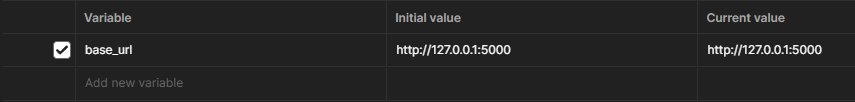
\includegraphics[width=0.8\textwidth]{Imagenes/baseURL.png}
  \caption{Variable \texttt{baseURL} en Postman}
  \label{fig:baseURL}
\end{figure}
Con la variable configurada, diseñé un flujo mínimo de peticiones para
verificar los principales endpoints de la API.  
Al inicio del proyecto el servidor carecía de interfaz web, por lo que toda la
validación se realizó a través de Postman: definía la petición, añadía los
parámetros necesarios y comprobaba la respuesta.  
Este ciclo de prueba–error permitió depurar la lógica hasta conseguir un
comportamiento estable.

Durante las primeras fases existían más endpoints de los que finalmente se han
publicado; algunos, como la creación de actores, siguen disponibles pero no
están expuestos en la aplicación web.

\begin{figure}[H]
  \centering
  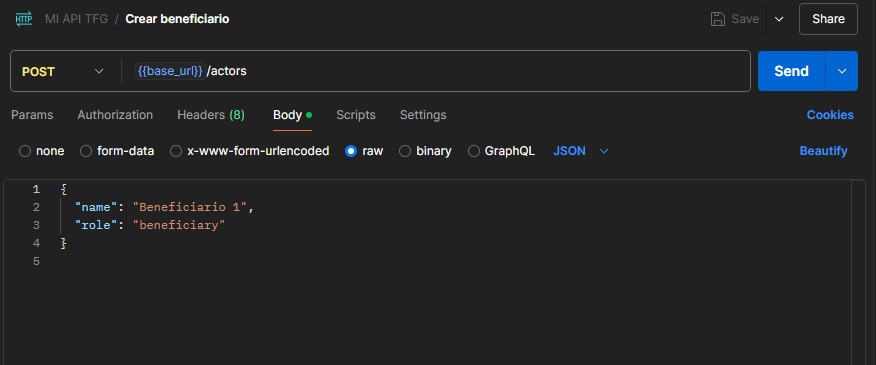
\includegraphics[width=0.8\textwidth]{Imagenes/crearActor.png}
  \caption{crearActor}
  \label{fig:crearActor}
\end{figure}

\begin{figure}[H]
  \centering
  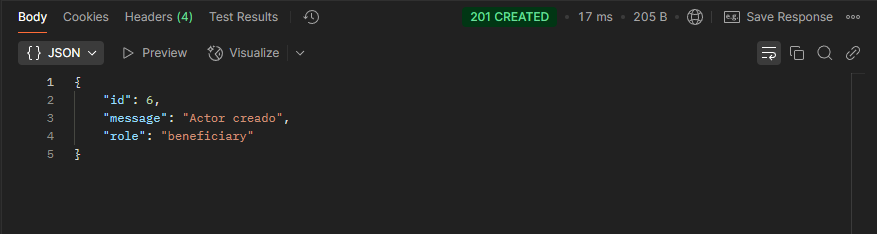
\includegraphics[width=0.8\textwidth]{Imagenes/crearActorResponse.png}
  \caption{crearActorResponse}
  \label{fig:crearActorResponse}
\end{figure}

Durante las primeras fases del desarollo se creó una coleccion de peticiones que se activa manualmente para verificar el correcto funcionamiento de la API tras cada cambio en las funcionalidades:

\begin{figure}[H]
  \centering
  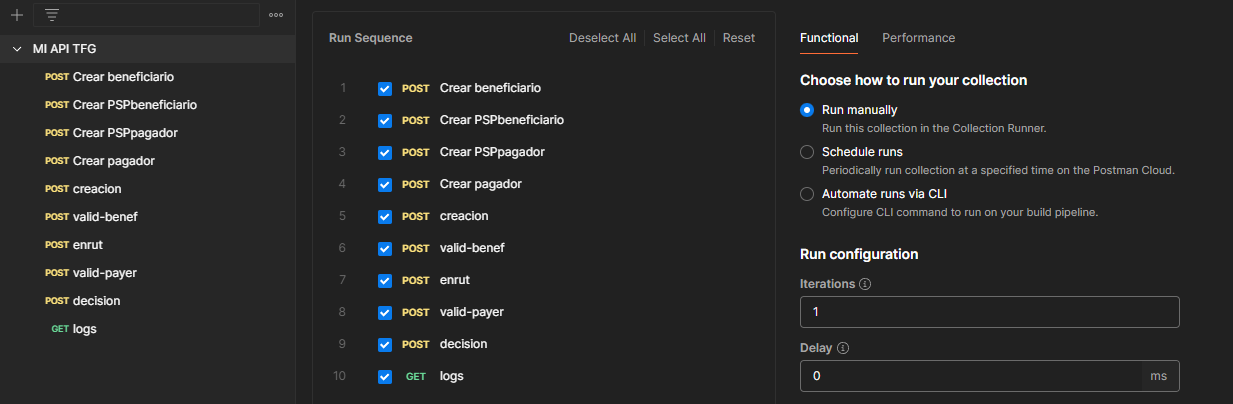
\includegraphics[width=0.8\textwidth]{Imagenes/MiAPITFG.png}
  \caption{MiAPITFG}
  \label{fig:MiAPITFG}
\end{figure}

\begin{figure}[H]
  \centering
  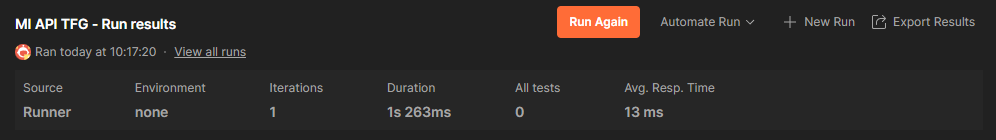
\includegraphics[width=0.8\textwidth]{Imagenes/RunResults.png}
  \caption{RunResults}
  \label{fig:RunResults}
\end{figure}

Las peticiones relevantes del flujo  son:

\begin{enumerate}
\item \textbf{Creación RTP}
    \begin{figure}[H]
    \centering
    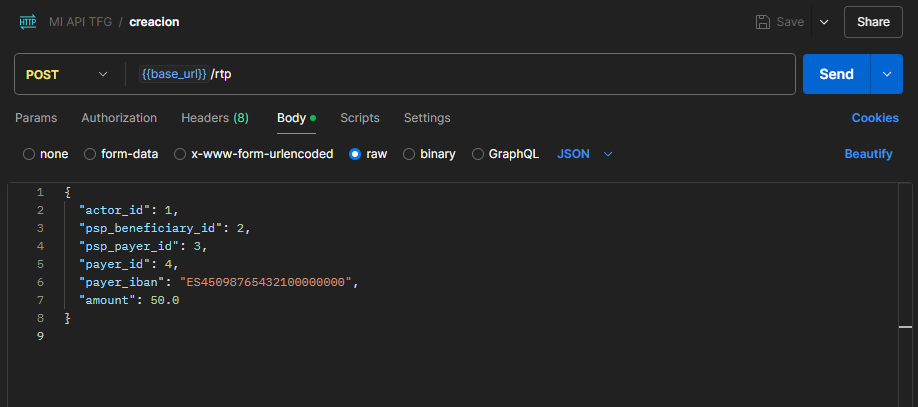
\includegraphics[width=0.8\textwidth]{Imagenes/crearRTP.png}
    \caption{crearRTP}
    \label{fig:crearRTP}
    \end{figure}

    \begin{figure}[H]
    \centering
    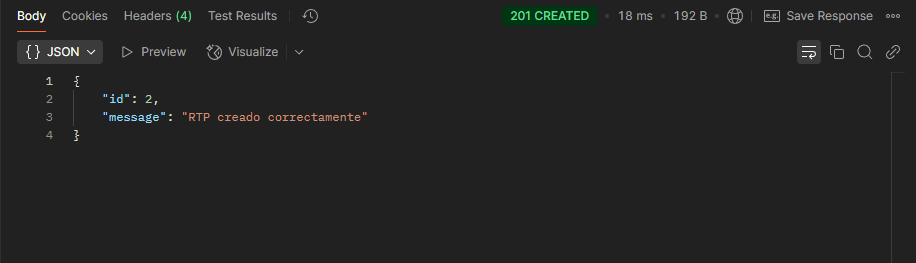
\includegraphics[width=0.8\textwidth]{Imagenes/crearRTPResponse.png}
    \caption{crearRTPResponse}
    \label{fig:crearRTPResponse}
    \end{figure}
\item \textbf{Validación y enrutado del PSP del beneficiario}
    \begin{figure}[H]
    \centering
    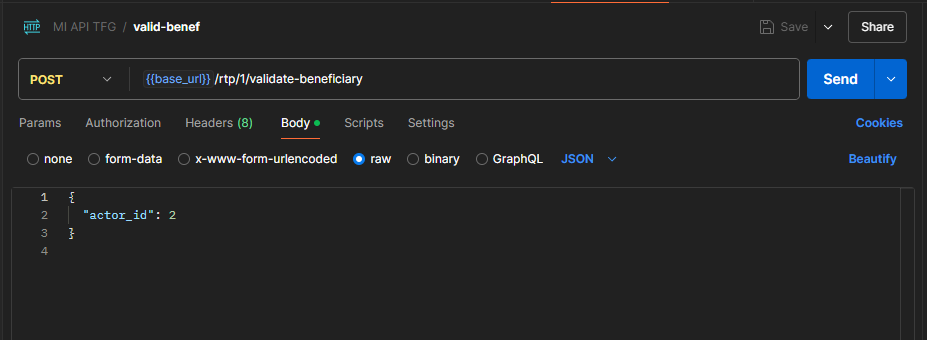
\includegraphics[width=0.8\textwidth]{Imagenes/validarBenef.png}
    \caption{validarBenef}
    \label{fig:validarBenef}
    \end{figure}

    \begin{figure}[H]
    \centering
    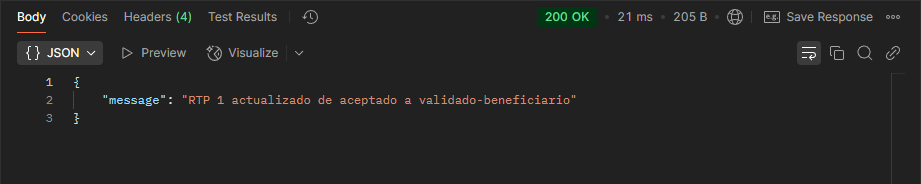
\includegraphics[width=0.8\textwidth]{Imagenes/validarBenefResponse.png}
    \caption{validarBenefResponse}
    \label{fig:validarBenefResponse}
    \end{figure}

    \begin{figure}[H]
    \centering
    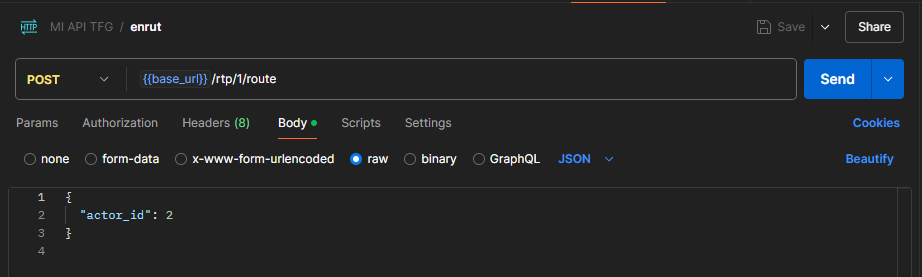
\includegraphics[width=0.8\textwidth]{Imagenes/enrutarBenef.png}
    \caption{enrutarBenef}
    \label{fig:enrutarBenef}
    \end{figure}


    \begin{figure}[H]
    \centering
    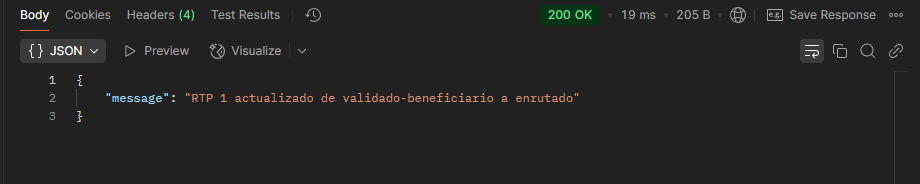
\includegraphics[width=0.8\textwidth]{Imagenes/enrutarBenefResponse.png}
    \caption{enrutarBenefResponse}
    \label{fig:enrutarBenefResponse}
    \end{figure}

\item \textbf{Validación del PSP del pagador}

    \begin{figure}[H]
    \centering
    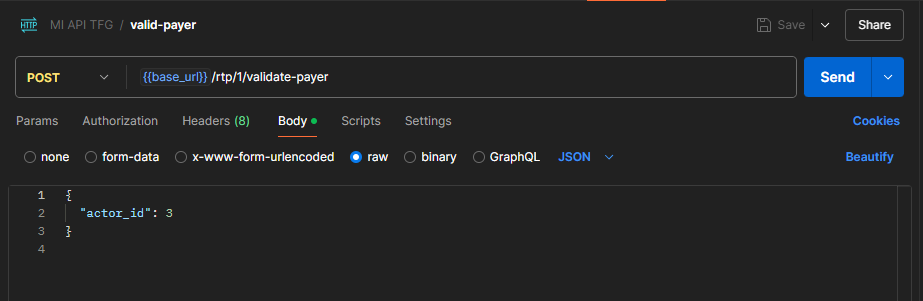
\includegraphics[width=0.8\textwidth]{Imagenes/validarPayer.png}
    \caption{validarPayer}
    \label{fig:validarPayer}
    \end{figure}

    \begin{figure}[H]
    \centering
    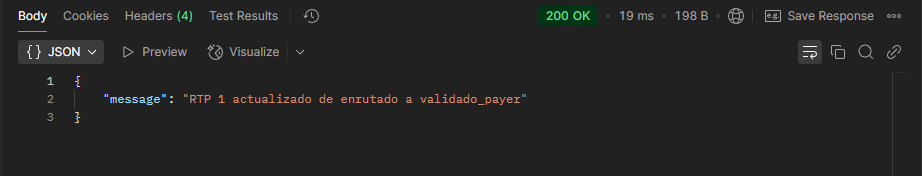
\includegraphics[width=0.8\textwidth]{Imagenes/validarPayerResponse.png}
    \caption{validarPayerResponse}
    \label{fig:validarPayerResponse}
    \end{figure}

\item \textbf{Decisión final}
\item 
    \begin{figure}[H]
    \centering
    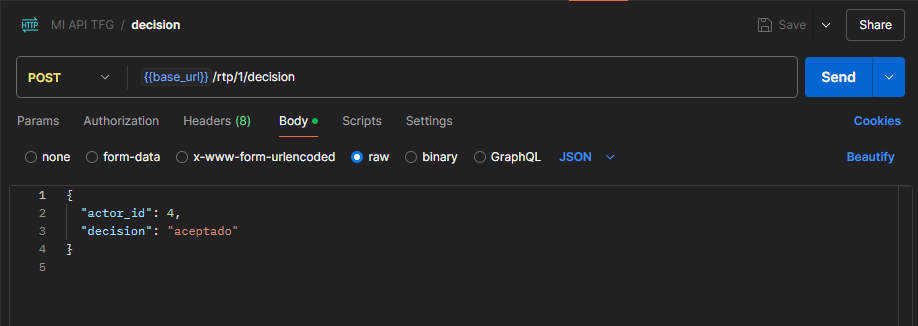
\includegraphics[width=0.8\textwidth]{Imagenes/decision.png}
    \caption{decision}
    \label{fig:decision}
    \end{figure}

    \begin{figure}[H]
    \centering
    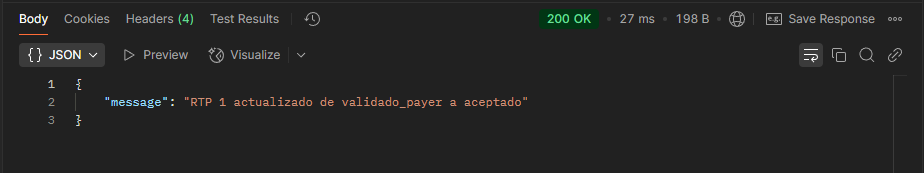
\includegraphics[width=0.8\textwidth]{Imagenes/decisionResponse.png}
    \caption{decisionResponse}
    \label{fig:decisionResponse}
    \end{figure}
\end{enumerate}

Hay ocasiones en las que el flujo no va a completarse debido a errores o rechazos:

Si al crear el RTP el IBAN no corresponde con ningún cliente regitrado en el esquema RTP o no cumple la normativa ISO 13616\footnote{Esta norma internacional define la estructura del IBAN: ES + 2 dígitos de control + 20 dígitos del número de cuenta}

    \begin{figure}[H]
    \centering
    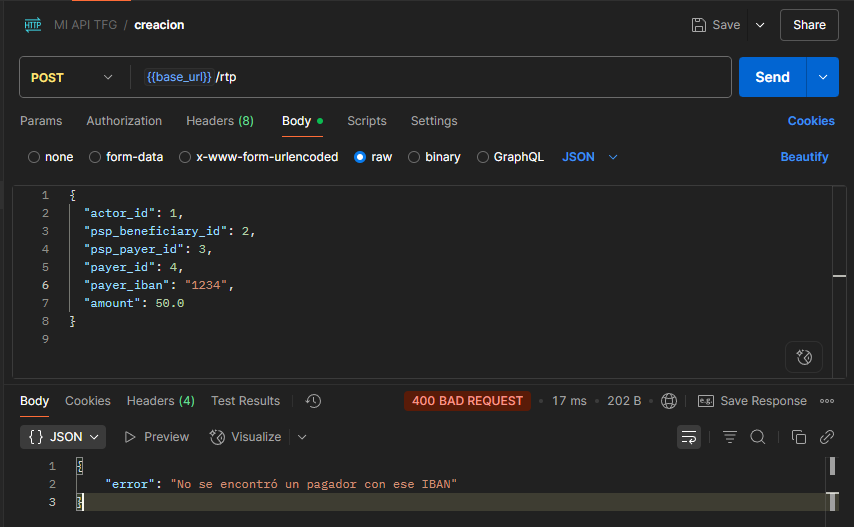
\includegraphics[width=0.8\textwidth]{Imagenes/error1.png}
    \caption{error1}
    \label{fig:error1}
    \end{figure}

Si se crea un RTP con importe mayor al que el pagador puede hacer frente, el RTP llegará hasta el PSP del pagador, quien tras comprobar el importe, lo rechazará.

    \begin{figure}[H]
    \centering
    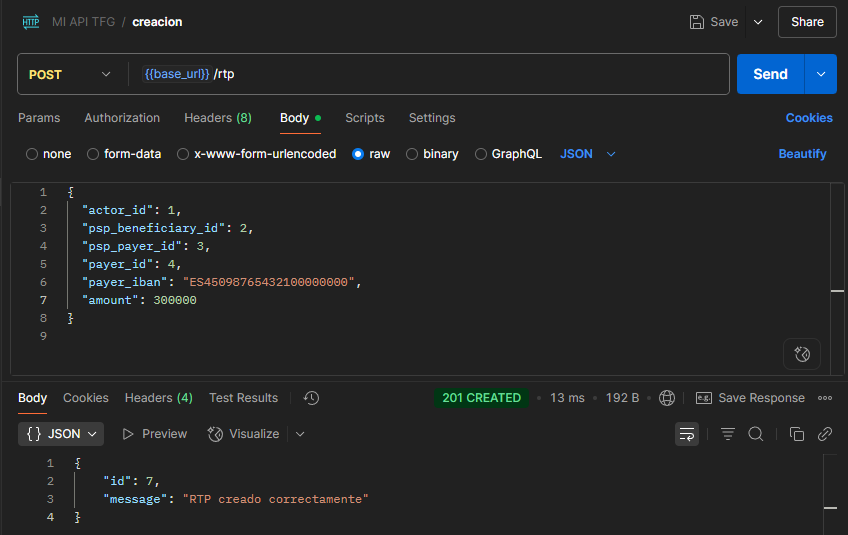
\includegraphics[width=0.8\textwidth]{Imagenes/error2_1.png}
    \caption{error2\_1}
    \label{fig:error2_1}
    \end{figure}

    \begin{figure}[H]
    \centering
    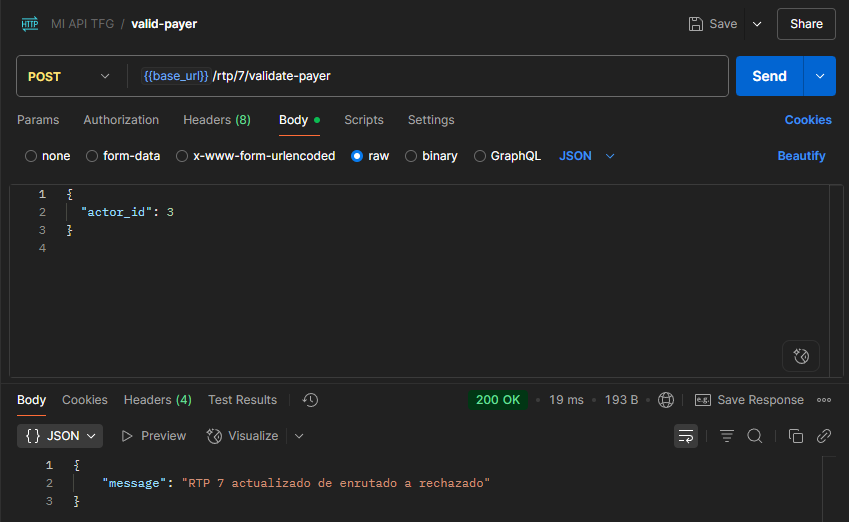
\includegraphics[width=0.8\textwidth]{Imagenes/error2_2.png}
    \caption{error2\_2}
    \label{fig:error2_2}
    \end{figure}

Cuando se crea un RTP deben existir los cuatro actores involucrados o de lo contrario también dará un error:

    \begin{figure}[H]
    \centering
    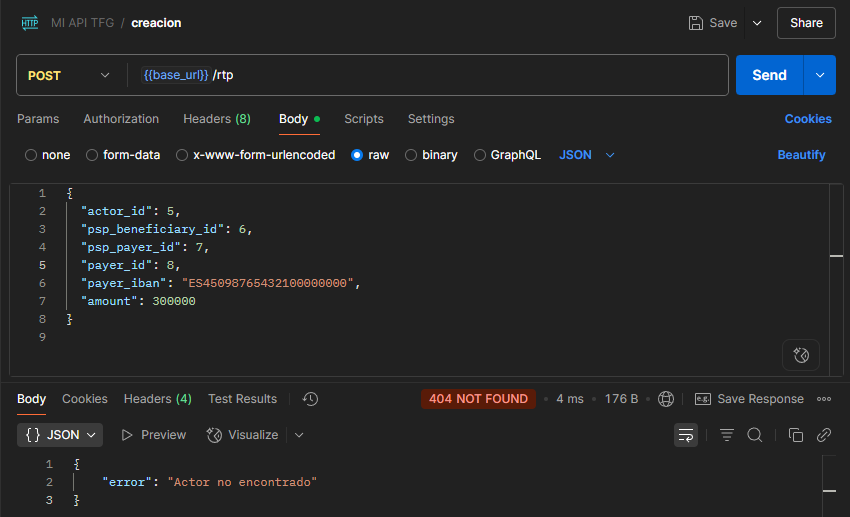
\includegraphics[width=0.8\textwidth]{Imagenes/error3.png}
    \caption{error3}
    \label{fig:error3}
    \end{figure}
